\documentclass[danish,a4paper,twocolumn,amsmath,amssymb,floatfix]{revtex4-1}
\usepackage[danish]{babel}
\renewcommand{\danishhyphenmins}{22}		%Giver mulighed for dansk orddeling. Slet kun hvis du VED hvad du laver, eller skal skrive noget på engelsk.
\usepackage[utf8]{inputenc}	%Hvis du benytter windows i stedet for linux, så skift utf8 ud med latin1. Tillader danske tegn.
\usepackage[T1]{fontenc}	%Tillader danske tegn
\usepackage{graphicx}		%Tillader indsættelse af billeder
\usepackage{dcolumn}		%Bruges til at lave matematiske tabelsøjler... se datatabel
\usepackage{booktabs}		%linjer i tabeller...
\usepackage{mathtools}		%Ekstra matematik... bare lad den være, du får muligvis brug for den.
\usepackage{siunitx}	%Bruges \SI{<tal>}{<enhed>}, \si{<enhed>} eller \num{<tal>}.
\sisetup{output-decimal-marker={,},separate-uncertainty=true}%Sørger for komma som decimalmarkør. Virker også ved decimaltal, hvis man bruger \num{<tal>}.
\usepackage{url}		 %bruges til at formattere url'er... kan sagtens udelades.
%Det følgende laver to makroer, \tref{} og \fref, der kan bruges ligesom \ref til at referere til hhv. tabeller og figurer. 
%De indsætter selv ordet Tabel/Figur, og sørger for at der ikke sker et linjebrud mellem dette og nummeret.
\newcommand{\tref}[1]{\tablename~\ref{#1}}
\newcommand{\fref}[1]{\figurename~\ref{#1}}
%Tilsvarende for ligninger. Indsætter "ligning (#)".
\newcommand{\lref}[1]{ligning~\eqref{#1}}
	% \eqref laver en reference med parenteser omkring (til brug ved ligninger.)
\newcommand{\picos}[0]{\textsc{PicoScope}} %hedder \picos for ikke at komme i kambolage med pico fra SIunits.
\newcommand{\epw}[0]{\textsc{EasyPlot}}    %epw er navnet på programfilen for easyplot, men det har ingen betydning for makroen. Jeg valgte det fordi det var noget jeg kunne huske, og det kan sagtens ændres.
\newcommand{\matl}[0]{\textsc{Matlab}} %Skriver Matlab med small caps.

%hyperref-pakken kan bruges til at redigere pdf-metadata. Det kan være et nice touch, men er generelt ikke påkrævet. Laver automatisk referencer i teksten til farvede hyperlinks i.
\usepackage{hyperref}
\hypersetup
{   pdfsubject={Rapport},
	pdfauthor={Anne Andersen}
    pdftitle={Røntgenøvelsen},
    pdfstartview=FitH,
    colorlinks=true}
    
%Følgende gør, at subscripts bliver ikke-kursiv. Anvendes X_|<subscript>|. Erstattes evt. med X_{\mathrm{<subscript>}}.
\makeatletter
\begingroup
\catcode`\_=\active
\protected\gdef_{\@ifnextchar|\subtextup\sb}
\endgroup
\def\subtextup|#1|{\sb{\textup{#1}}}
\AtBeginDocument{\catcode`\_=12 \mathcode`\_=32768 }
\makeatother

\usepackage[danish=quotes]{csquotes} %Danske citationstegn. \enquote{}

%Lad disse to linjer være. De sørger for at bunden af siden bliver pæn, og fjerner indryk ved afsnit.
\raggedbottom
\parindent = 0pt

\begin{document}

%Dette er boksen i toppen. Lad den være.
\framebox[\textwidth][l]{\textbf{
\begin{tabular}{p{\linewidth}l}
Received date:  & {Approved:}\\
& Date:\\
& Signature:\\
(reserved for instructor) & \\
\end{tabular}
}}
%Boksen slutter her.

\bigskip
\title{Experimental Physics III, Experiment 2: X-rays}

\author{Anne Andersen}%Forfatter 1
 \altaffiliation{Institut for Fysik og Astronomi, Aarhus Universitet, Danmark} %Hvis begge personer studerer det samme sted, kan informationen her flyttes til \affiliation
\author{Børge Børgesen}%Forfatter 2
\altaffiliation{Kemisk Institut, Aarhus Universitet, Danmark} 
\affiliation{Team number $\pi$} %Det er nok de færreste der er så priviligerede at have holdnummer pi, så skift denne tekst ud
	% Bemærk at det har betydning hvor \affilliation og \altaffiliation er placeret i forhold til \author. De virker på alle forfattere der kommer før dem.
\date{January 1st 2018} %Dato. Husk at ændre!

\begin{abstract}
\bigskip


Her kommer det såkaldte \enquote{abstract} hvor du kort og klart beskriver øvelsens indhold og dine hovedresultater. Det skal ikke være særlig langt, men bør kunne læses som en selvstående tekst, der giver en potentiel læser et godt indtryk af indholdet af den følgende rapport.
\end{abstract}

\maketitle

\noindent
\section*{Introduction}



\section*{Materials and Methods}


\begin{figure}
%OBS:
%Hvis man bruger TeXnicCenter under windows til editering af TeX filer,
%kan man ikke inkludere .eps grafik filer ved konvertering til .pdf.
%Man kan i stedet anvende f.eks. .jpg eller .png filer
\centering
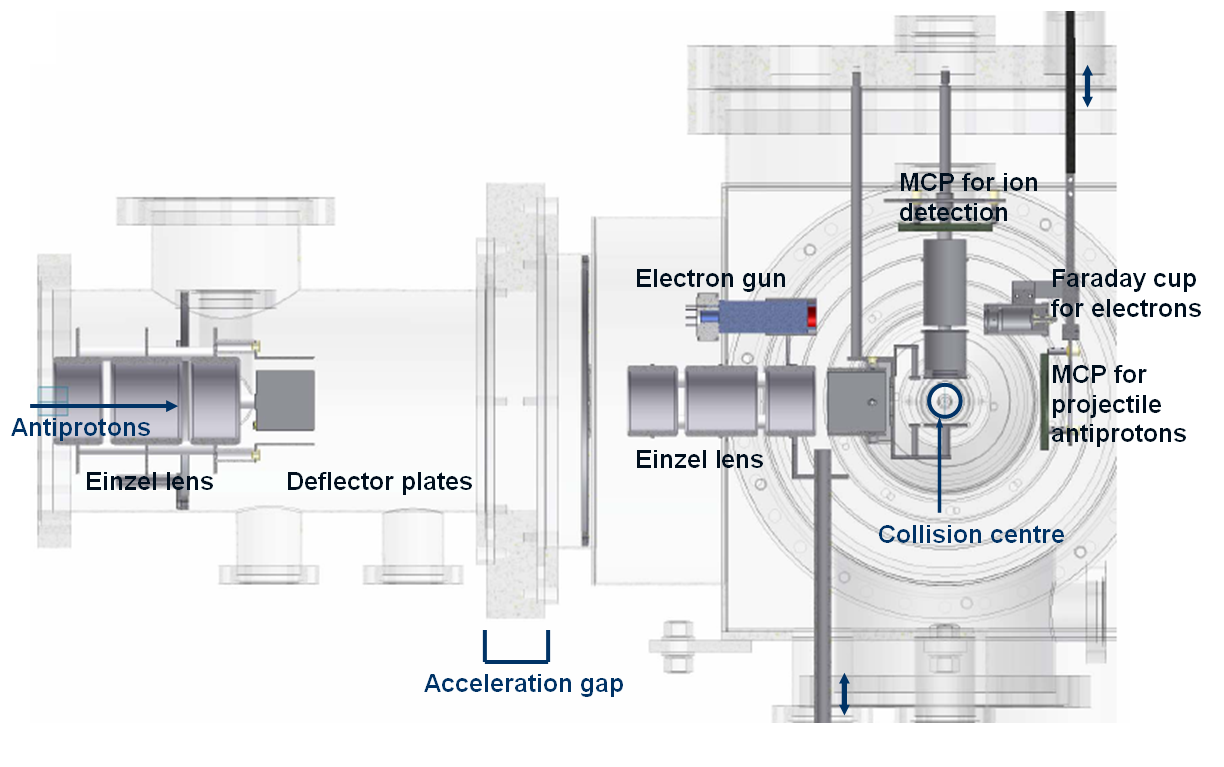
\includegraphics[width=\columnwidth]{figure1.png}
\caption{\sl Opstilling til første del af øvelsen. Her ses....}
\label{fig:en_label} %Bruges til referencer. Husk at den SKAL stå efter den tilhørende "\caption{}"
\end{figure} 

\subsection*{Results}



\begin{table}[h]
%I denne tabel bruger jeg søjletypen D{#1}{#2}{#3} fra pakken dcolumn. Denne sætter hele søjlen i matematik-mode, og justerer
%indholdet, således at #1 bliver justeret over hinanden. I det færdige output bliver #1 erstattet med #2. og i #3 angiver man antallet af 
%tegn før og efter #1 (syntax: før.efter).
%\multicolumn{#4}{#5}{#6} tillader at forhindre matematikmode i en række. #4 giver antallet af søjler der skal kombineres, her 1 eller 2, #5 giver den søjlejustering der skal gælde, her c, og #6 giver det der skal stå i feltet.
% koden @{$\pm$} udskifter et søjlemellemrum med et plus-minus tegn, således at data angives i en søjle og usikkerhederne i den næste. Generelt udskifter @{#7} søjlemellemrum ud med #7.
% *{#8}{#9} bruges til at gentage #9 det antal gange som #8 angiver, her 2.
\centering
\caption{\sl De målte data for kalibreringen af....}%Tabelforklaringer placeres normalt over tabellen.
\begin{tabular}{l D{.}{,}{1.2} *{2}{ D{.}{,}{1.2} @{$\pm$} D{.}{,}{1.2} } D{.}{,}{1.3}}
\toprule
  & \multicolumn{1}{c}{E (\si{\mega\electronvolt})} & \multicolumn{2}{c}{I (\si{\ampere})} & \multicolumn{2}{c}{V (\si{\milli\volt})} & \multicolumn{1}{c}{K (\si{\centi\meter})} \\
\midrule
aaaa  &  3.44  &  1.23 & 0.03  &  3.67 & 0.04  &  0.012 \\
bbbb  &  2.44  &  1.45 & 0.05  &  2.89 & 0.02  &  0.023 \\
cccc  &  1.44  &  2.67 & 0.02  &  3.99 & 0.07  &  0.089 \\
\bottomrule
\end{tabular}
\label{tbl:eksempel}
\end{table}


\begin{figure*} %Det er stjernen der gør forskellen. Husk at den også skal være i \end.
	\centering
	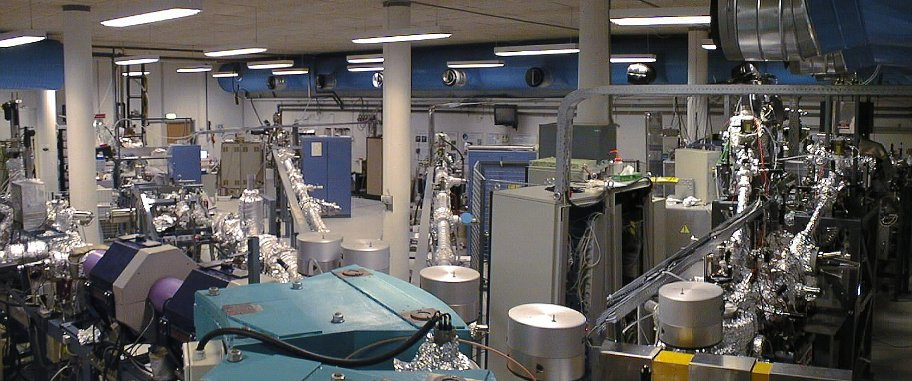
\includegraphics[width=\textwidth]{figure2.jpg}
	\caption{\sl Benyt denne kommando hvis du skal indsætte en figur som er for bred til at kunne være i en enkelt kolonne. Virker tilsvarende for tabeller.}
\end{figure*} 

\begin{equation}
	A = \sum_i (n - \frac{a_i}{b_i})
\end{equation}

\subsection*{Discussion}

\begin{figure}
	\centering
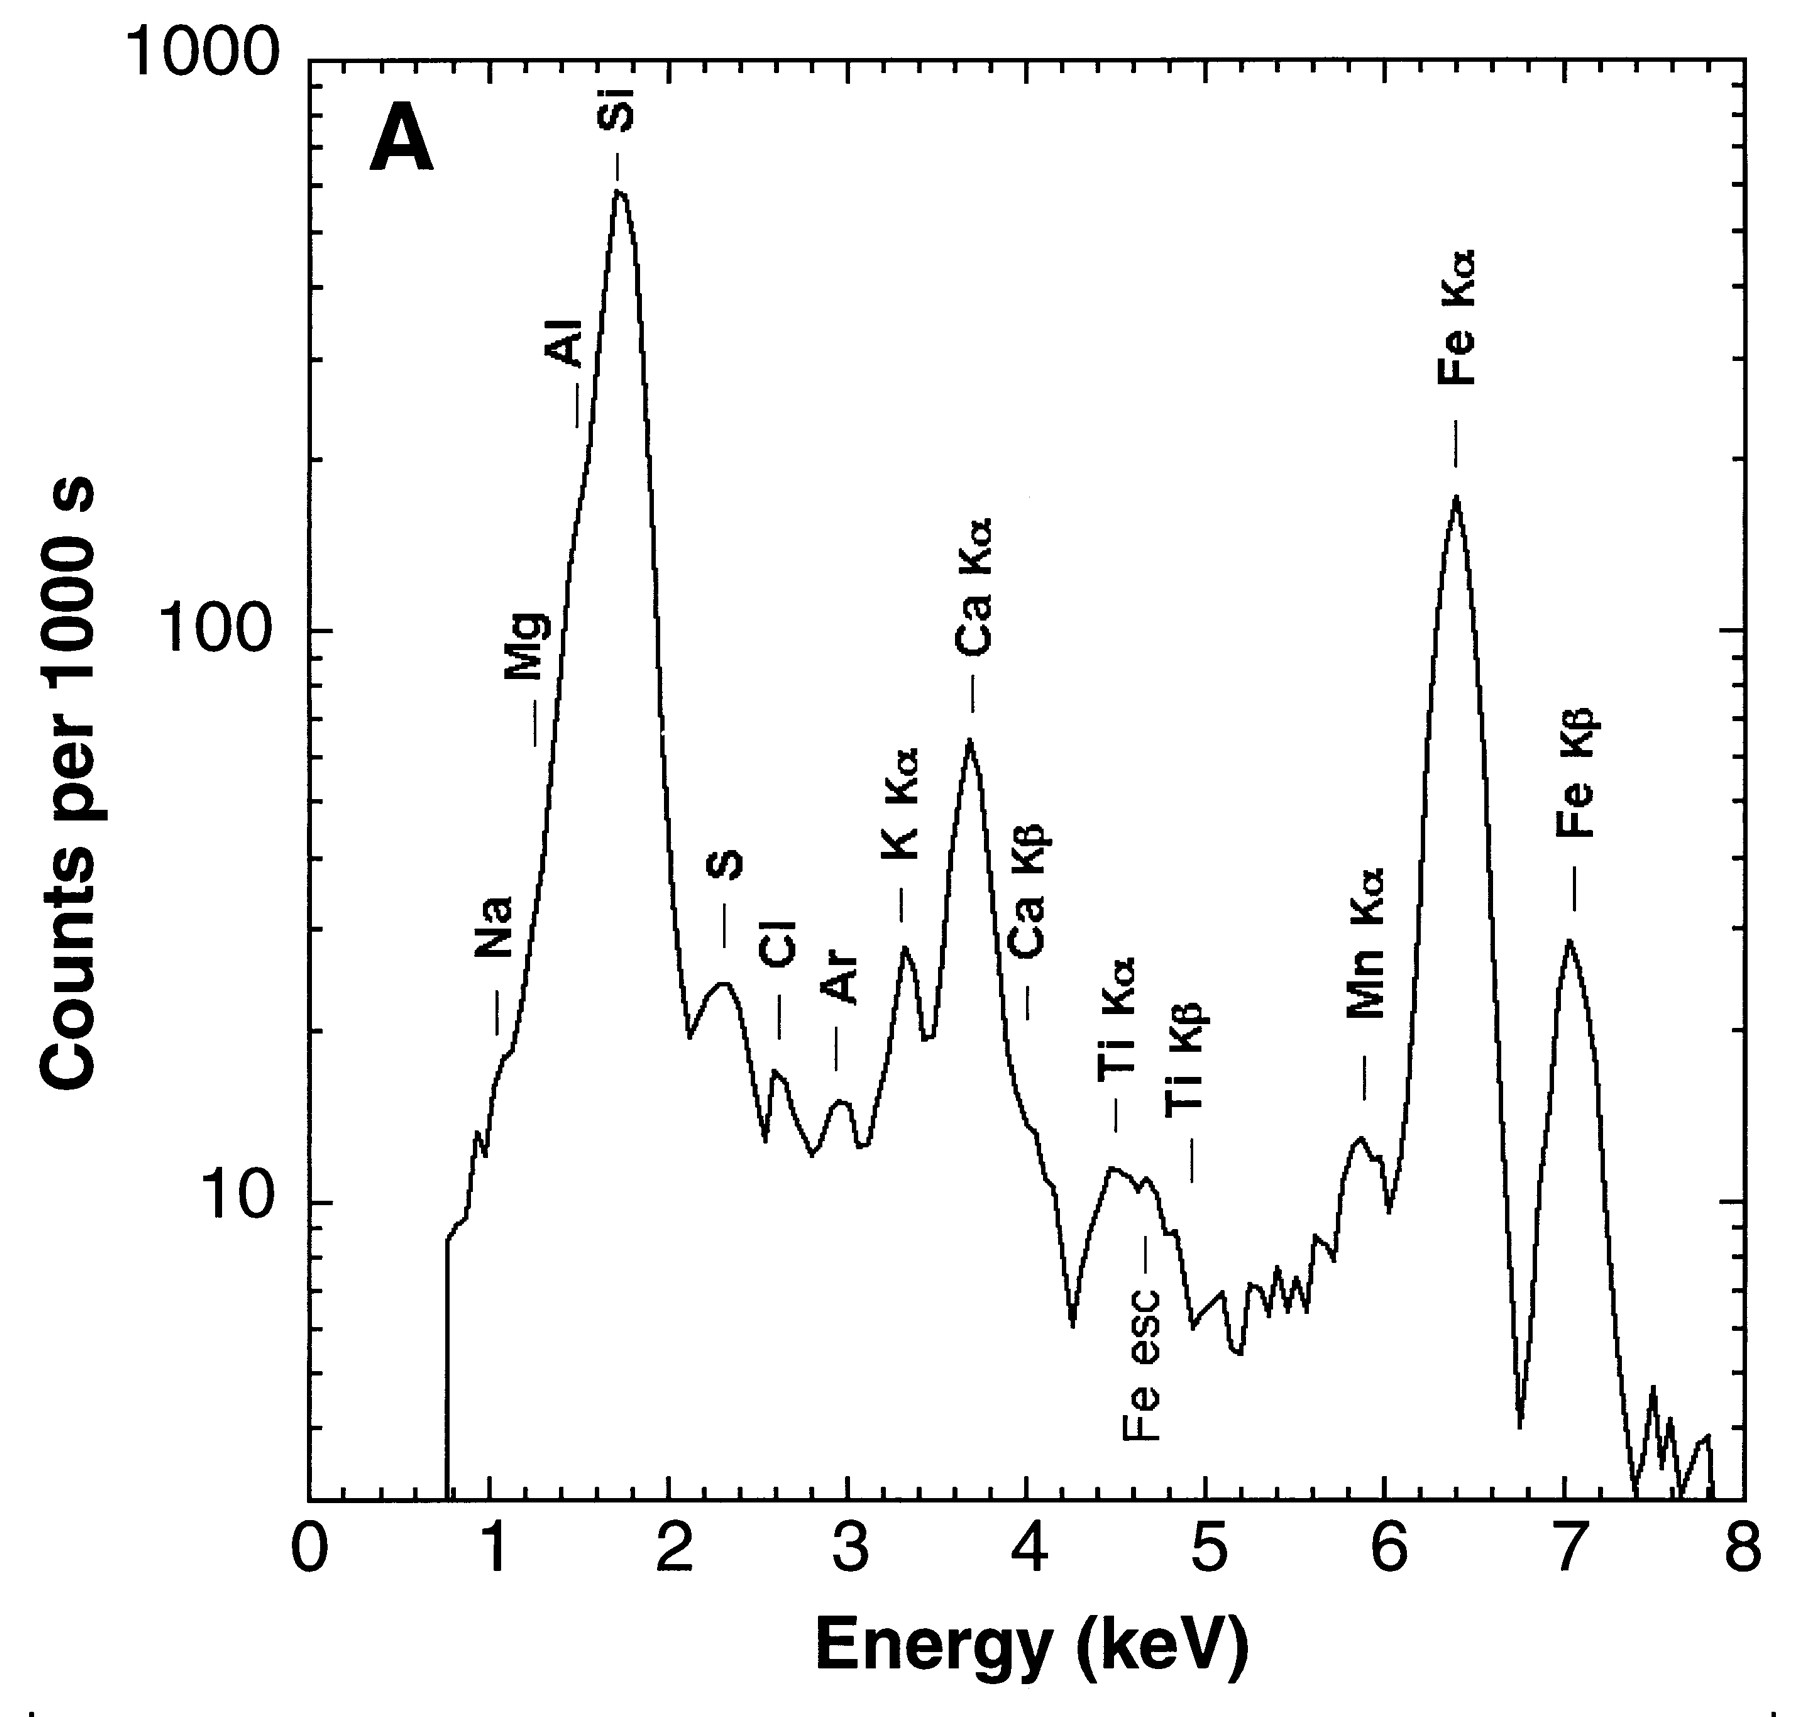
\includegraphics[width=0.9\columnwidth]{figure3.jpg}
\caption{Energikalibrering}
\label{fig:kalibrering}
\end{figure}

\section*{Conclusion}

\appendix
\section*{Bemærkninger}
\textsl{ Denne template (skabelon) er ment som en rettesnor for rapportens indhold og udseende. De enkelte afsnit og deres rækkefølge skal selvfølgelig tilpasses den enkelte øvelse. Det er derimod vigtigt at du holder dig til layout (skrifttyper, marginer, kolonner,...), som en øvelse i at skrive rapporter og artikler hvor designet ofte er forudbestemt. Af hensyn til rettelses-proceduren bedes du beholde \enquote{kassen} over overskriften. Denne \LaTeX-template bygger på REVTeX 4.1--pakken fra The American Physical Society, og er blevet tilpasset af Peter Birk Nielsen (mindre revision 2013 af Jonas Refsgaard). For mere info om \LaTeX{}, se Daleif \cite{Daleif}}

\begin{thebibliography}{99}
\section*{REFERENCES}

\bibitem{hk:1}
Eksperimentelle øvelser i fysik, øvelsesvejledninger efteråret 2006, IFA, Aarhus Universitet
\bibitem{hk:2}
	Se: \url{www.inkscape.com}
\bibitem{Daleif}
	Dalifs bog om \LaTeX. \url{http://www.imf.au.dk/system/latex/bog/version3beta.html}

\end{thebibliography}

\end{document}

